\documentclass{beamer}
\usetheme{CambridgeUS}
\usepackage[utf8]{inputenc}
%\usepackage{default}

%\setbeamertemplate{footline}[frame number]

\setbeamertemplate{headline}
{
    \leavevmode%
    \hbox{%
        \begin{beamercolorbox}[wd=.75\paperwidth,ht=0.001ex,dp=1ex,center]{ }%
            \usebeamerfont{ } 
        \end{beamercolorbox}%
        \begin{beamercolorbox}[wd=.28\paperwidth,ht=0.001ex,dp=1ex,right]{ }%
            \usebeamerfont{ }\hspace*{2em}
             / \hspace*{2ex}
        \end{beamercolorbox}}%
        \vskip0pt%
    }

\setbeamertemplate{footline}
{
    \leavevmode%
    \hbox{%
        \begin{beamercolorbox}[wd=.28\paperwidth,ht=2.25ex,dp=1ex,center]{author in head/foot}%
            \usebeamerfont{author in head/foot}\insertshortauthor{}
        \end{beamercolorbox}%
        \begin{beamercolorbox}[wd=.28\paperwidth,ht=2.25ex,dp=1ex,right]{date in head/foot}%
            \usebeamerfont{date in head/foot}\insertshortdate{}\hspace*{2em}
            \insertframenumber{} / \inserttotalframenumber\hspace*{2ex} 
        \end{beamercolorbox}}%
        \vskip0pt%
    }

\author{Unai Aseguinolaza Aguirreche}
\title{Anharmonic effects in thermoelectric and 2D materials}
\institute{Supervided by Aitor Bergara and Ion Errea}
\date{\today}
\titlegraphic{
\includegraphics[width=.35\textwidth,height=.25\textheight]{Pictures/LOGOS/EHU.jpg}
              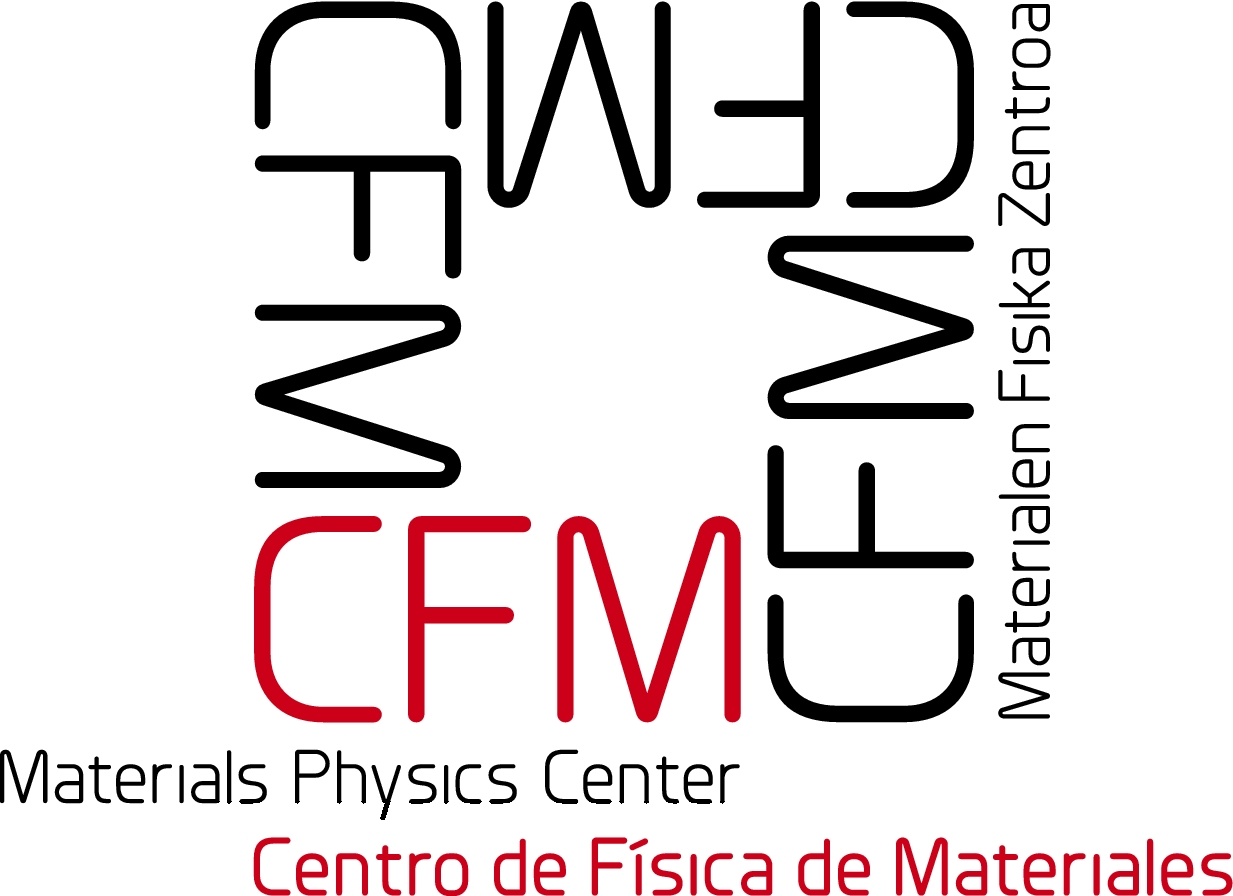
\includegraphics[width=.25\textwidth,height=.3\textheight]{Pictures/LOGOS/CFM.jpg}
              
\includegraphics[width=.35\textwidth,height=.2\textheight]{Pictures/LOGOS/DIPC.jpg}}

\begin{document}

\setbeamertemplate{navigation symbols}{}

%%%%%%%%%%%%%%%%%%%%%%%%%%%%%%%%%%%%%%%%%%%%%%%%%%%%%%%%%%%%%%%%%%%%%%%%%%%%%%%%%%

\begin{frame}
 \titlepage
\end{frame}

\begin{frame}

\frametitle{General outline}
\begin{enumerate}
	\item Thermoelectric monochalcogenides (part 1)
	\begin{itemize}
		\item Bulk SnSe and SnS
		\item Monolayer SnSe
	\end{itemize}
	\vspace{2cm}
\item 2D materials (part 2)
	\begin{itemize}
		\item Graphene
	\end{itemize}
\end{enumerate}

\end{frame}

%%%%%%%%%%%%%%%%%%%%%%%%%%%%%%%%%%%%%%%%%%%%%%%%%%%%%%%%%%%%%%%%%%%%%%%%%%%%%%%%%%%%%

\begin{frame}

\frametitle{Outline}
\begin{itemize}
\item Introduction
\vspace{0.5cm}
\item Theoretical framework
\vspace{0.5cm}
\item Part 1: Thermoelectric monochalcogenides
\vspace{0.5cm}
\item Part 2: 2D materials
\vspace{0.5cm}
\item Conclusions
\end{itemize}

\end{frame}

%%%%%%%%%%%%%%%%%%%%%%%%%%%%%%%%%%%%%%%%%%%%%%%%%%%%%%%%%%%%%%%%%%%%%%%%%%%%%%%%%%%%%%%

\begin{frame}

\frametitle{Introduction}
\vspace{-0.5cm}
\begin{equation}
ZT=\frac{S^{2}\sigma T}{\kappa}, \hspace{0.6cm} S=-\frac{\Delta V}{\Delta T}%, \hspace{0.6cm} ZT_{ave}=\frac{1}{T_{h}-T_{c}}\int_{T_{c}}^{T_{c}}ZTdT
\nonumber
\end{equation}
\begin{center}
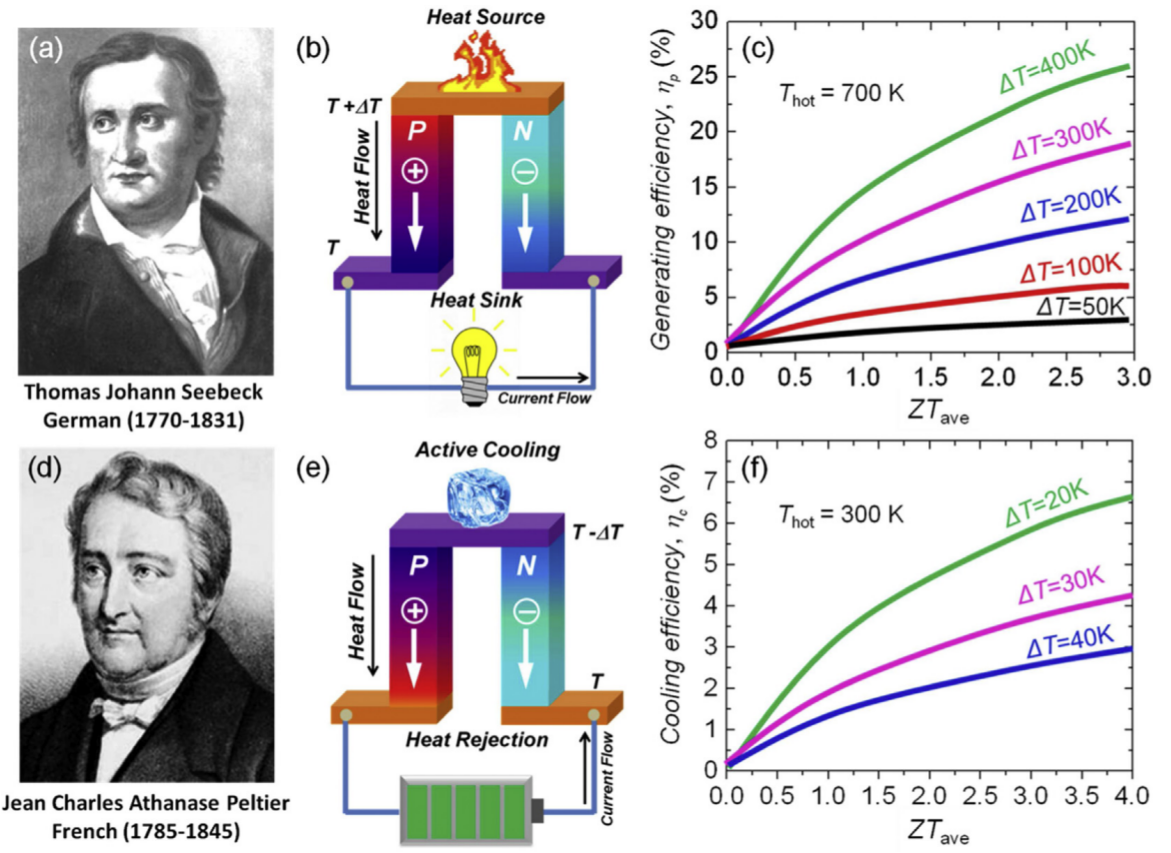
\includegraphics[width=0.7\linewidth]{Pictures/INTRO/generation-cooling.png}
\end{center}
\vspace{-0.1cm}
\begin{tiny}
X. Zhang, L-D. Zhao / Journal of Materiomics 1 (2015) 92-105
\end{tiny}

\end{frame}

%%%%%%%%%%%%%%%%%%%%%%%%%%%%%%%%%%%%%%%%%%%%%%%%%%%%%%%%%%%%%%%%%%%%%%%%%%%%%%%%%%%%%%

\begin{frame}

\frametitle{Introduction}
\vspace{-0.5cm}
\begin{center}
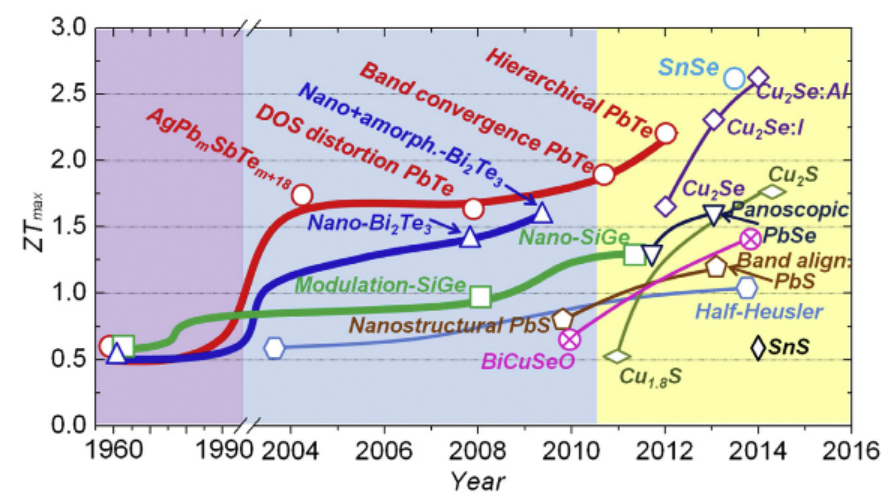
\includegraphics[width=0.7\linewidth]{Pictures/INTRO/ztvstemp.png}
\end{center}
\vspace{-0.1cm}
\begin{itemize}
\item $ZT_{max}$ low and in narrow temperature ranges
\item Very limited technological applications.
\end{itemize}
\begin{tiny}
X. Zhang, L-D. Zhao / Journal of Materiomics 1 (2015) 92-105
\end{tiny}

\end{frame}

%%%%%%%%%%%%%%%%%%%%%%%%%%%%%%%%%%%%%%%%%%%%%%%%%%%%%%%%%%%%%%%%%%%%%%%%%%%%%%%%%%%%%%%%

\begin{frame}

\frametitle{Introduction}
\vspace{-0.5cm}
\begin{center}
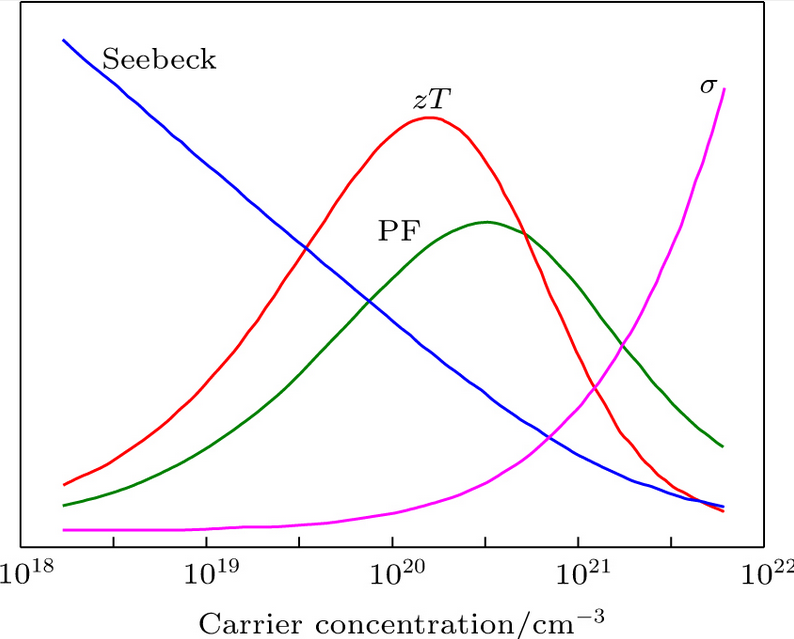
\includegraphics[width=0.5\linewidth]{Pictures/INTRO/decoupling.png}
\end{center}
\vspace{-0.1cm}
\begin{itemize}
\item The physical magnitudes that define $ZT$ are correlated
\item How to overcome:
	\begin{itemize}
	\item Doping + nanostructuring
	\item Proximity to phase transitions
	\item \dots
	\end{itemize}
\end{itemize}

\end{frame}

%%%%%%%%%%%%%%%%%%%%%%%%%%%%%%%%%%%%%%%%%%%%%%%%%%%%%%%%%%%%%%%%%%%%%%%%%%%%%%%%%%%%%%%%%

\begin{frame}

\frametitle{Introduction}
\vspace{-0.5cm}
\begin{center}
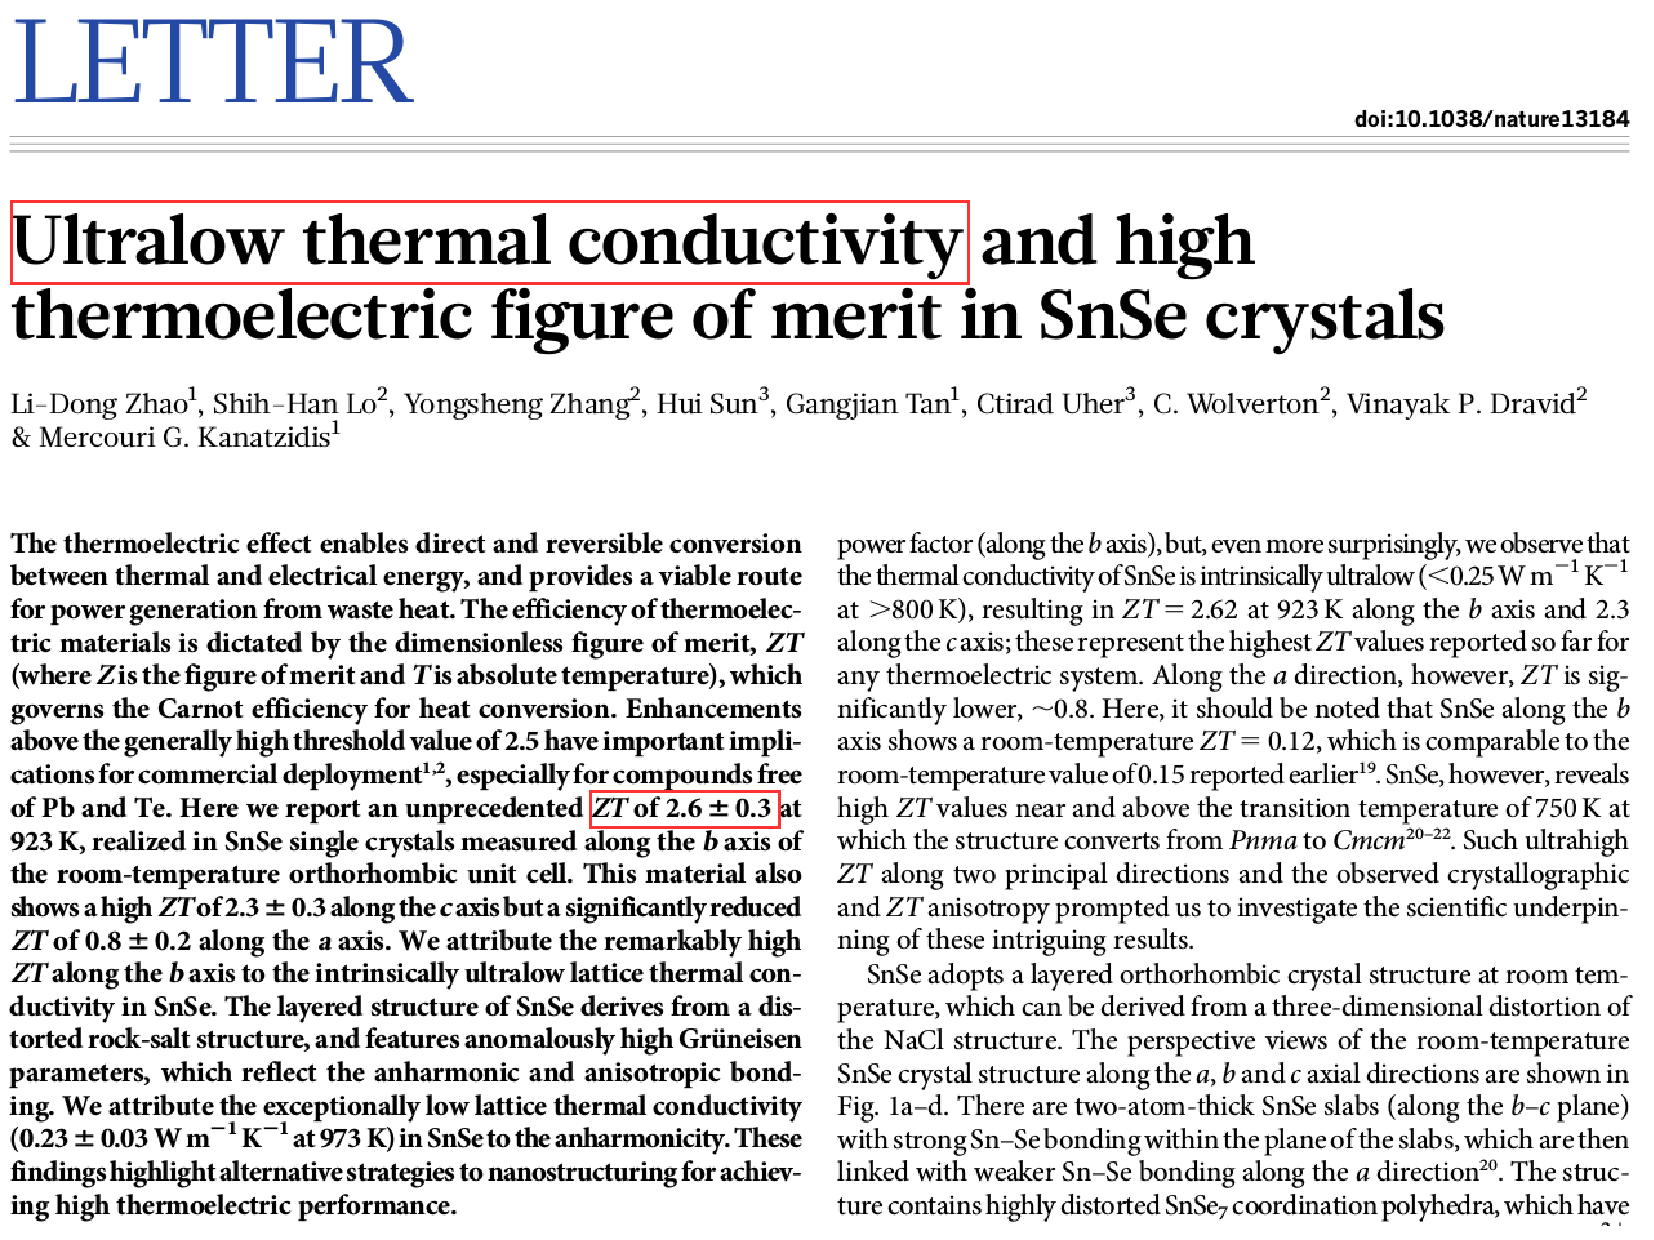
\includegraphics[width=0.7\linewidth]{Pictures/INTRO/natureSnSe.pdf}
\end{center}
\begin{itemize}
\item The best thermoelectric material so far: Intrinsic semiconductor with low lattice thermal 
conductivity ($\kappa=\kappa_{el} + \kappa_{l}$) 
\end{itemize}

\end{frame}

%%%%%%%%%%%%%%%%%%%%%%%%%%%%%%%%%%%%%%%%%%%%%%%%%%%%%%%%%%%%%%%%%%%%%%%%%%%%%%%%%%%%%%%%%%%

\begin{frame}

\frametitle{Introduction}
\vspace{-0.5cm}
\begin{center}
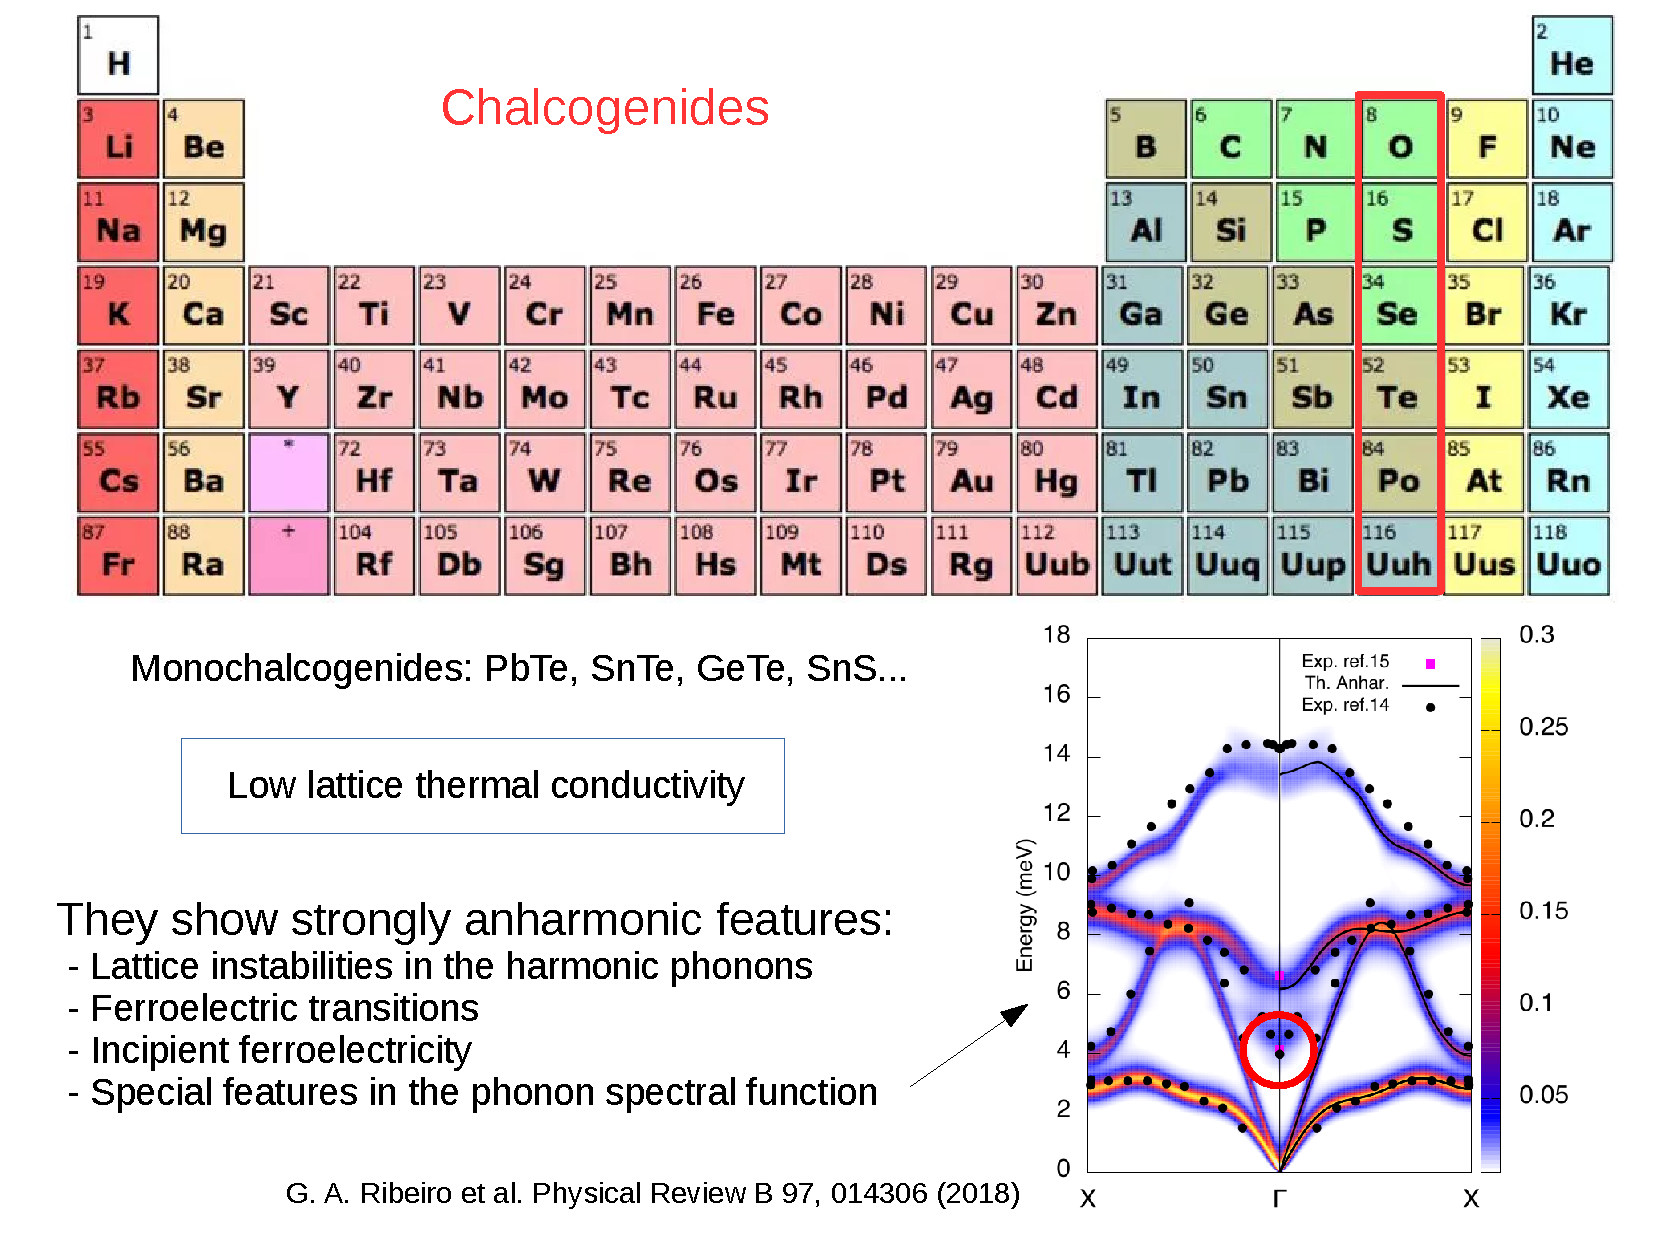
\includegraphics[width=0.85\linewidth]{Pictures/INTRO/chalcogenides.pdf}
\end{center}

\end{frame}

%%%%%%%%%%%%%%%%%%%%%%%%%%%%%%%%%%%%%%%%%%%%%%%%%%%%%%%%%%%%%%%%%%%%%%%%%%%%%%%%%%%%%%%%%%%%%%%

%\begin{frame}
%
%\frametitle{Introduction}
%\vspace{-0.5cm}
%\begin{center}
%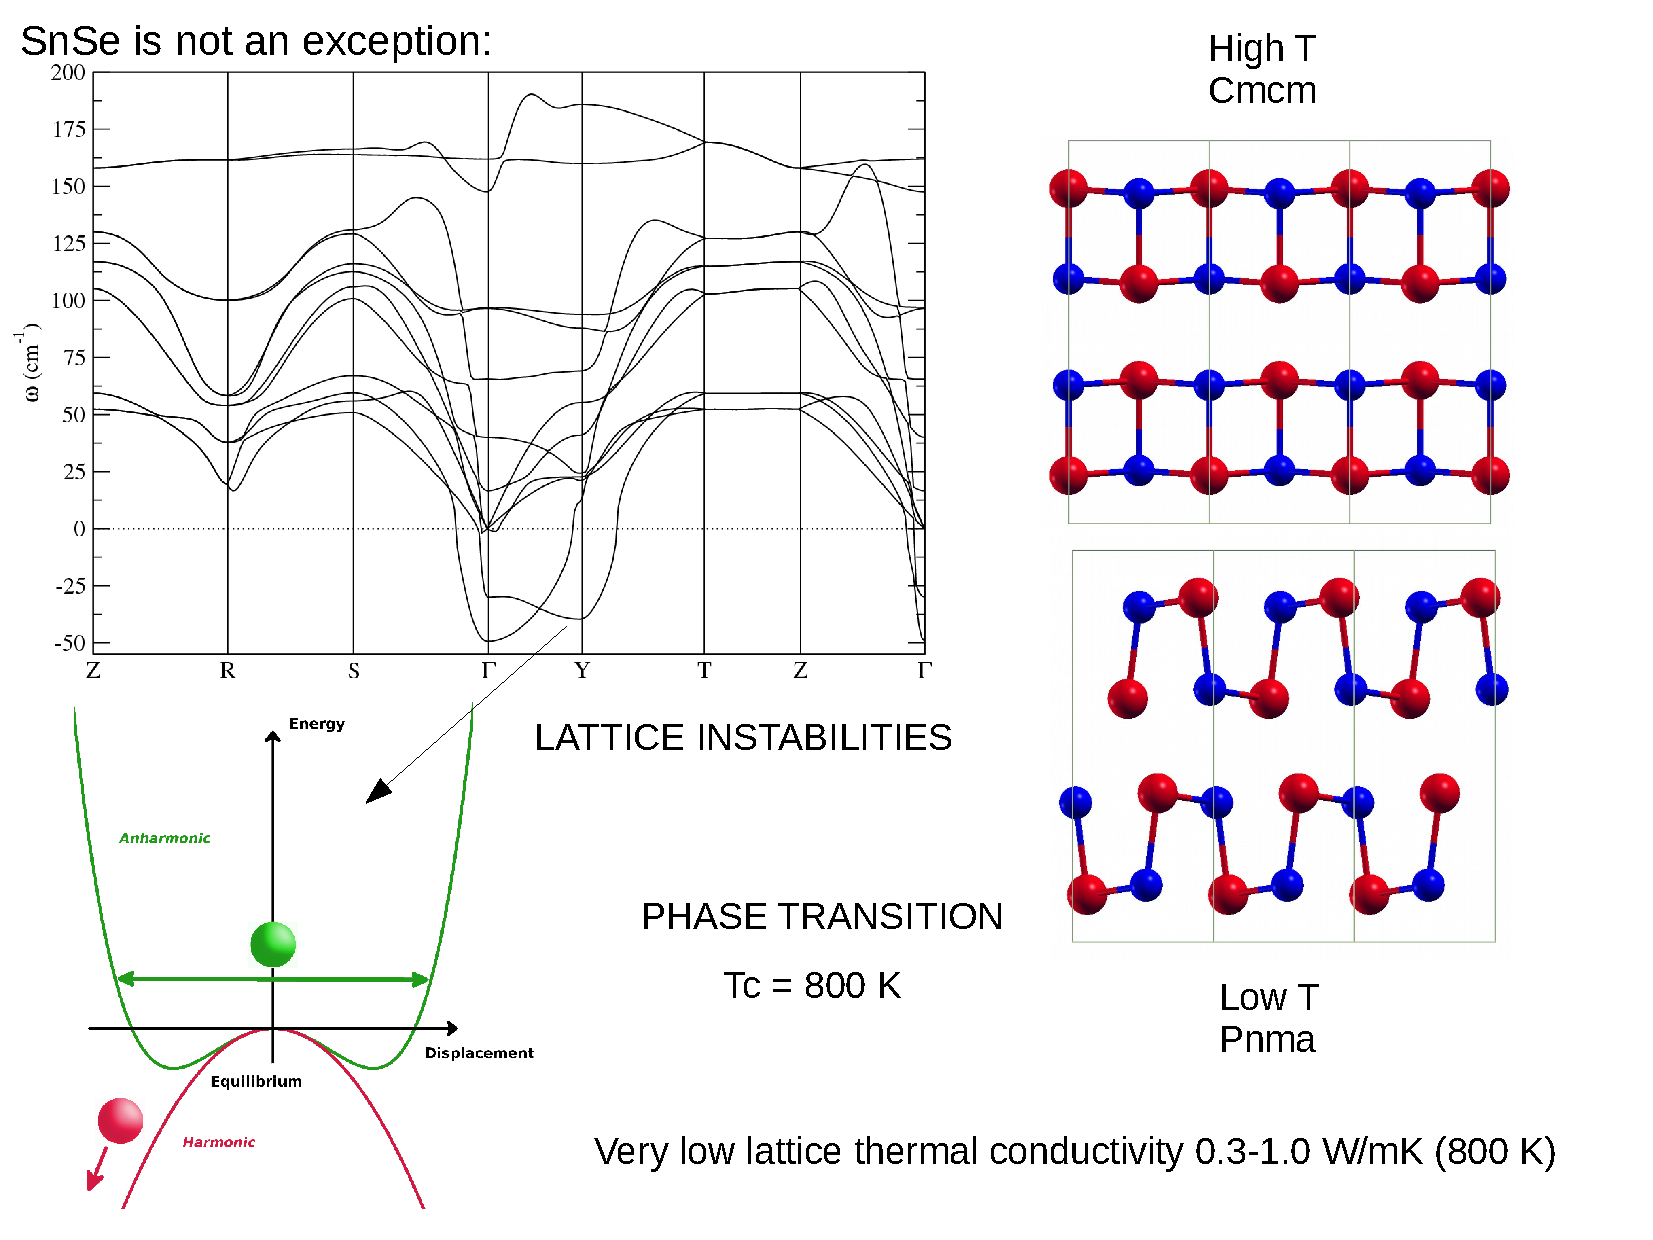
\includegraphics[width=0.85\linewidth]{Pictures/INTRO/SnSeIntro.pdf}
%\end{center}
%
%\end{frame}

%%%%%%%%%%%%%%%%%%%%%%%%%%%%%%%%%%%%%%%%%%%%%%%%%%%%%%%%%%%%%%%%%%%%%%%%%%%%%%%%%%%%%%%%%%%%%%%%%%

\begin{frame}

\frametitle{Theoretical framework}
\vspace{-0.1cm}
 \begin{itemize}
  \item Ionic Hamiltonian
 \end{itemize}
 \begin{equation}
  \nonumber
  H=T+V(\boldsymbol{R})
 \end{equation}
where $\boldsymbol{R}=\boldsymbol{R}_{0}+\boldsymbol{u}$.
\begin{itemize}
 \item Assuming that $V(\boldsymbol{R})$ is well reproduced by a quadratic potential in the range of $\boldsymbol{u}$, Taylor expand the potential
\end{itemize}
\begin{equation}
 \nonumber
 V(\boldsymbol{R})\simeq V(\boldsymbol{R}_{0}) + \frac{1}{2}\sum_{ab}\phi_{ab}u_{a}u_{b} + O(u^{3})
\end{equation}
where $\phi_{ab}=\partial^{2}V/\partial u_{a}\partial u_{b}|_{0}$.
\begin{equation}
 \nonumber
 V^{harm}(\boldsymbol{R})= V(\boldsymbol{R}_{0}) + \frac{1}{2}\sum_{ab}\phi_{ab}u_{a}u_{b} 
\end{equation}
\begin{itemize}
 \item This Hamiltonian (Harmonic Hamiltonian) can be solved exactly.
 \item It provides well defined phonon quasiparticles
\end{itemize}
\begin{equation}
 \nonumber
 \sum_{b}\phi_{ab}\epsilon^{b}_{\mu}=M\omega_{\mu}^{2}\epsilon^{a}_{\mu}
\end{equation}

\end{frame}

%%%%%%%%%%%%%%%%%%%%%%%%%%%%%%%%%%%%%%%%%%%%%%%%%%%%%%%%%%%%%%%%%%%%%%%%%%%%%%%%%%%%%%%%%%%

\begin{frame}

 \frametitle{Anharmonic theory: SSCHA}
\begin{columns}
\begin{column}{0.45\textwidth}
 \begin{itemize}
  \item \color{red}{Harmonic approximation}:
  \begin{itemize}
   \item It does not work in monochalcogenides because they show harmonic instabilities.
  \end{itemize}
 \end{itemize}
 \begin{itemize}
  \item \color{red}{Perturbative approaches are not an option.}
  \begin{itemize}
   \item They are built on top of the harmonic theory.
  \end{itemize}
 \end{itemize}
\end{column}
\begin{column}{0.45\textwidth}
 \begin{center}
  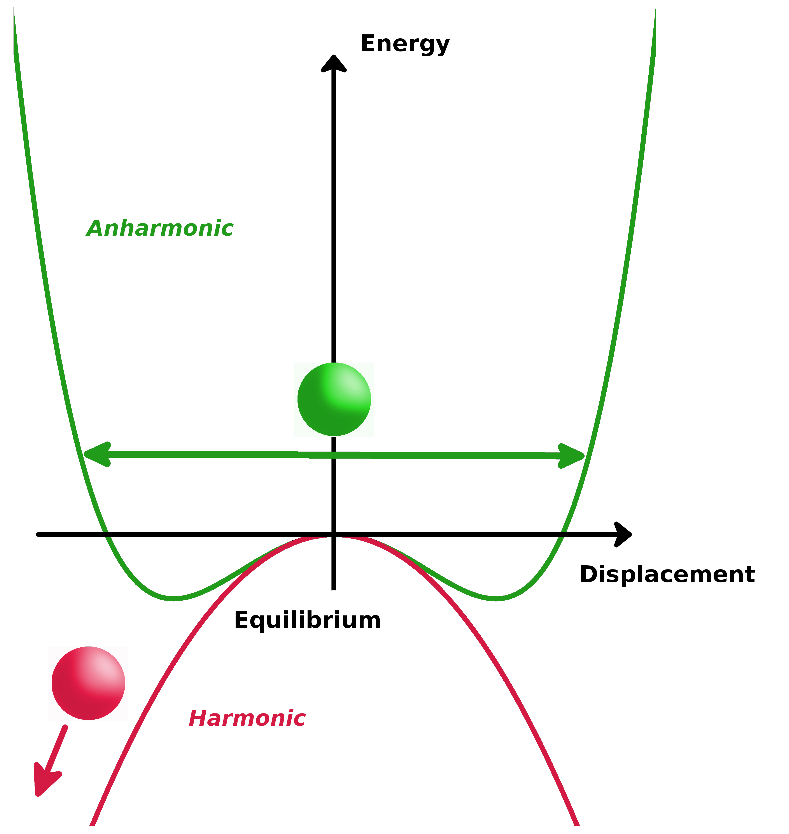
\includegraphics[width=0.9\linewidth]{Pictures/THEORY/instability.png}
 \end{center}
\end{column}
\end{columns}
\begin{itemize}
  \item \color{teal}{We apply a variational non-perturbative approach with anharmonic terms to infinite order: Stochastic self-consistent harmonic
  approximation (SSCHA)}
\end{itemize}
 \begin{tiny}
  I. Errea et al. Physical Review Letters 111 (17), 177002 (2013)
 \end{tiny}
 \begin{tiny}
  R. Bianco et al. Physical Review B 96, 014111 (2017)
 \end{tiny}

\end{frame}

%%%%%%%%%%%%%%%%%%%%%%%%%%%%%%%%%%%%%%%%%%%%%%%%%%%%%%%%%%%%%%%%%%%%%%%%%%%%%%%%%%%%%%%%%%%%%%

\begin{frame}

\frametitle{Theoretical framework}
 \begin{itemize}
  \item SCHA is a method for approximating the vibrational free energy of a crystal.
 \end{itemize}
\begin{equation}
 \nonumber
 F_{H}=tr(\rho_{H}H)+\frac{1}{k_{B}T}tr(\rho_{H}ln\rho_{H}) 
\end{equation}
\begin{equation}
 \nonumber
 \mathcal{F}_{H}[\mathcal{H}]=tr(\rho_{\mathcal{H}}H)+\frac{1}{k_{B}T}tr(\rho_{\mathcal{H}}ln\rho_{\mathcal{H}})=F_{\mathcal{H}}+\langle V-\mathcal{V}\rangle_{\rho_{\mathcal{H}}} 
\end{equation}
\begin{equation}
 \nonumber
 F_{H}\le\mathcal{F}_{H}[\mathcal{H}] 
\end{equation}
\begin{itemize}
	\item We take a harmonic trial density matrix $\rho_{\mathcal{H}}\equiv\rho_{\mathcal{H}}(\boldsymbol{\Phi},\boldsymbol{\mathcal{R}})$. Variables $\boldsymbol{\Phi}$ (SCHA/auxiliary phonons) and $\boldsymbol{\mathcal{R}}$ atomic centroids.
 \item The SCHA provides the harmonic density matrix that minimizes the free energy.
\end{itemize}

\end{frame}

%%%%%%%%%%%%%%%%%%%%%%%%%%%%%%%%%%%%%%%%%%%%%%%%%%%%%%%%%%%%%%%%%%%%%%%%%%%%%%%%%%%%%%%%%%%%%%%%

\begin{frame}

\frametitle{Theoretical framework}
\begin{itemize}
\item Landau Theory of second-order phase transitions
\end{itemize}
\begin{center}
\includegraphics[width=0.8\linewidth]{Pictures/THEORY/transition.eps}
\end{center}

\end{frame}

%%%%%%%%%%%%%%%%%%%%%%%%%%%%%%%%%%%%%%%%%%%%%%%%%%%%%%%%%%%%%%%%%%%%%%%%%%%%%%%%%%%%%%%%%%%%%%%%%%

\begin{frame}

\frametitle{Theoretical framework}
\begin{itemize}
 \item The free energy is a well defined quantity within the SCHA.
 \item For a given temperature, experimentally measured phonon frequencies will be centered in the phonon frequencies defined by $\partial^{2}\mathcal{F}/\partial\boldsymbol{\mathcal{R}}^{2}$.
\end{itemize}
\begin{equation}
\nonumber
 \frac{\partial^{2}\mathcal{F}}{\partial\boldsymbol{\mathcal{R}}\partial\boldsymbol{\mathcal{R}}}=\boldsymbol{\Phi}+\overset{(3)}{\boldsymbol{\Phi}}\Lambda[\boldsymbol{1}-\overset{(4)}{\boldsymbol{
 \Phi}}\Lambda]^{-1}\overset{(3)}{\boldsymbol{\Phi}}
\end{equation}
\begin{itemize}
 \item $\overset{(3)}{\boldsymbol{\Phi}}=\left\langle\frac{\partial^{3}V}{\partial\boldsymbol{R}^{3}}\right\rangle_{\rho_{\mathcal{H}}}$, \hspace{0.2cm}
       $\overset{(4)}{\boldsymbol{\Phi}}=\left\langle\frac{\partial^{4}V}{\partial\boldsymbol{R}^{4}}\right\rangle_{\rho_{\mathcal{H}}}$, and
       $\Lambda\equiv\Lambda(\boldsymbol{\Phi})$.
\end{itemize}

\end{frame}

%%%%%%%%%%%%%%%%%%%%%%%%%%%%%%%%%%%%%%%%%%%%%%%%%%%%%%%%%%%%%%%%%%%%%%%%%%%%%%%%%%%%%%%%%%%%%%%%

\begin{frame}

 \frametitle{Theoretical framework}
 \begin{itemize}
 \item The static theory can be expanded by a dynamical ansatz.
 \end{itemize}
 \begin{equation}
 \sigma(\mathbf{q},\omega)=\frac{1}{\pi}\times\sum_{\mu}\frac{-\omega Im\Pi_{\mu}(\mathbf{q},\omega)}{(\omega^{2}-\omega_{\mu}^{2}
 (\mathbf{q})-Re\Pi_{\mu}(\mathbf{q},\omega))^{2}+(Im\Pi_{\mu}(\mathbf{q},\omega))^{2}}
 \nonumber
 \end{equation}
 \begin{center}
  \includegraphics[width=0.65\linewidth]{Pictures/THEORY/ins-toy1.eps}
 \end{center}

\end{frame}

%%%%%%%%%%%%%%%%%%%%%%%%%%%%%%%%%%%%%%%%%%%%%%%%%%%%%%%%%%%%%%%%%%%%%%%%%%%%%%%%%%%%%%%%%%%%%%%%

\begin{frame}

\frametitle{Theoretical framework}
\begin{equation}
\nonumber
\mathcal{Z}_{\mu}(\mathbf{q},\omega)=\sqrt{\omega_{\mu}^{2}(\mathbf{q})+\Pi_{\mu}(\mathbf{q},\omega+i0^{+})}
\end{equation}
\begin{equation}
\nonumber
 \Omega_{\mu}(\mathbf{q})=Re\mathcal{Z}_{\mu}(\mathbf{q},\omega_{\mu}(\mathbf{q})),
\end{equation}
\begin{equation}
\nonumber
 \Gamma_{\mu}(\mathbf{q})=-Im\mathcal{Z}_{\mu}(\mathbf{q},\omega_{\mu}(\mathbf{q}))
\end{equation}
\begin{center}
  \includegraphics[width=0.6\linewidth]{Pictures/THEORY/ins-toy2.eps}
 \end{center}

\end{frame}

%%%%%%%%%%%%%%%%%%%%%%%%%%%%%%%%%%%%%%%%%%%%%%%%%%%%%%%%%%%%%%%%%%%%%%%%%%%%%%%%%%%%%%%%%%%%%%%%%

\begin{frame}

\frametitle{Theoretical framework}
\begin{itemize}
 \item The Lorentzian definition of phonons provides a straightforward way of calculating the lattice thermal conductivity
\end{itemize}
\begin{equation}
\nonumber
 \kappa_{l}=\frac{1}{N_{\mathbf{q}}\Omega_{cell} k_{B}T^{2}}\sum_{\mathbf{q}\mu}v_{\mu}(\mathbf{q})^{2}\omega_{\mu}(\mathbf{q})^{2}n_{B}(\omega_{\mu}(\mathbf{q}))[n_{B}(\omega_{\mu}(\mathbf{q}))+1]\tau_{\mu}(\mathbf{q}).
\end{equation}

Summary:
\begin{itemize}
\item Anharmonic free energy
\item Phase transition temperature
\item Anharmonic phonons
\item Lattice thermal conductivity
\end{itemize}

\end{frame}

%%%%%%%%%%%%%%%%%%%%%%%%%%%%%%%%%%%%%%%%%%%%%%%%%%%%%%%%%%%%%%%%%%%%%%%%%%%%%%%%%%%%%%%%%%%%%%%%%

\begin{frame}

\frametitle{SnSe}
\begin{center}
  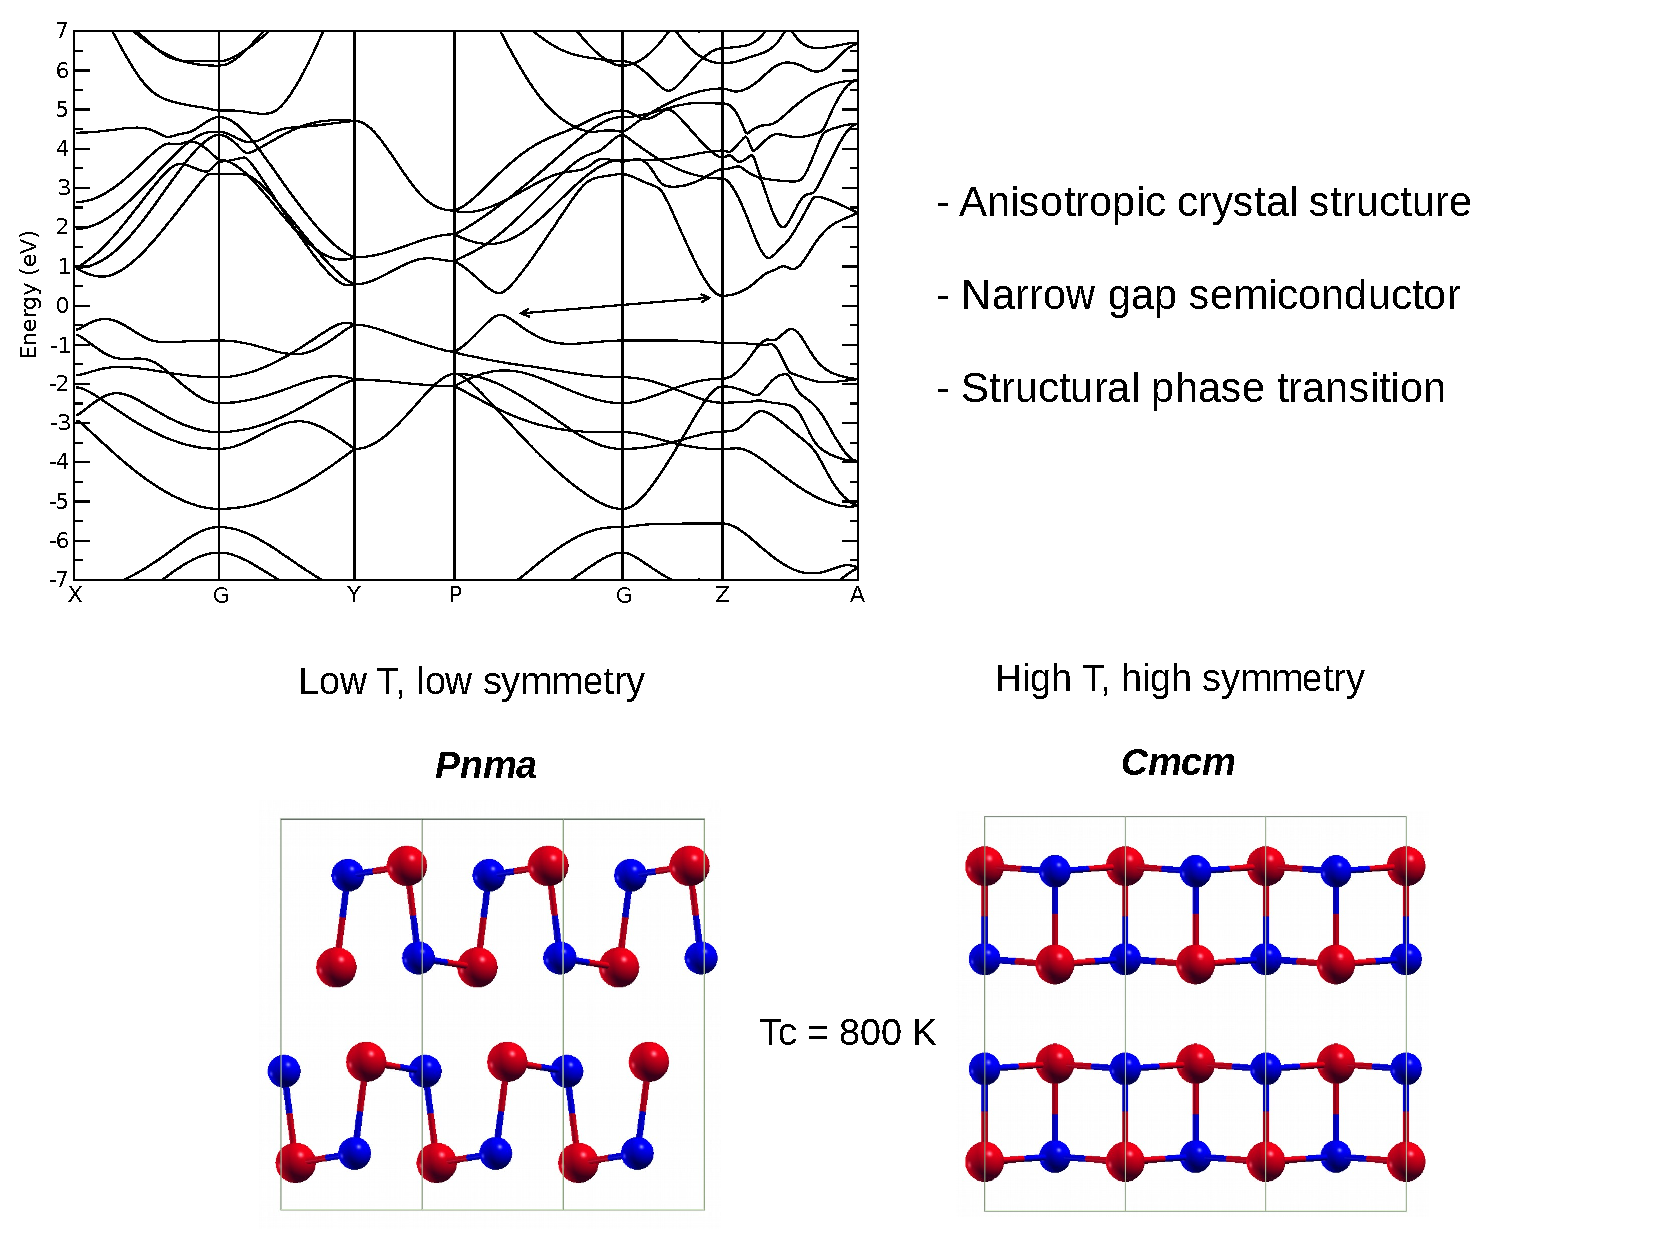
\includegraphics[width=0.85\linewidth]{Pictures/SnSe/figure1.pdf}
\end{center}

\end{frame}

%%%%%%%%%%%%%%%%%%%%%%%%%%%%%%%%%%%%%%%%%%%%%%%%%%%%%%%%%%%%%%%%%%%%%%%%%%%%%%%%%%%%%%%%%%%%%%%%%

\begin{frame}

\frametitle{SnSe}
\begin{center}
  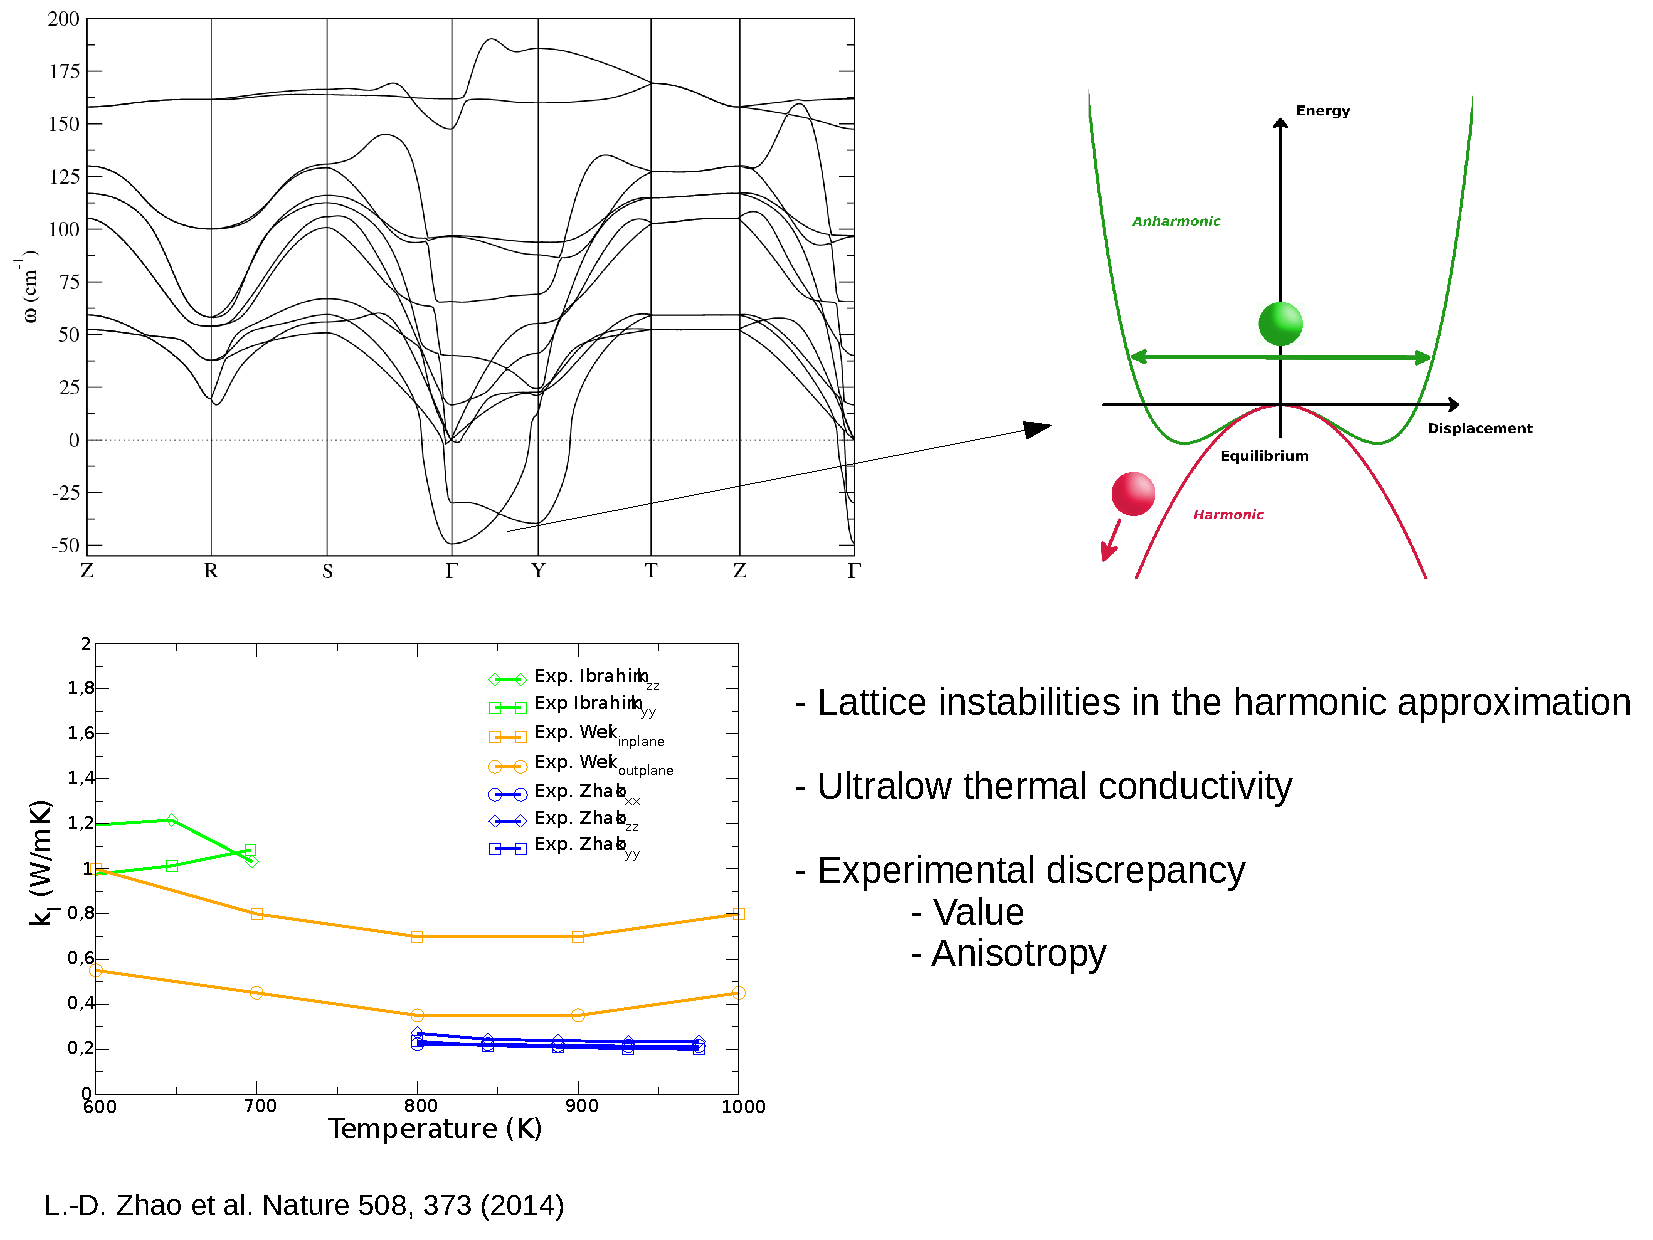
\includegraphics[width=0.85\linewidth]{Pictures/SnSe/figure2.pdf}
\end{center}

\end{frame}

%%%%%%%%%%%%%%%%%%%%%%%%%%%%%%%%%%%%%%%%%%%%%%%%%%%%%%%%%%%%%%%%%%%%%%%%%%%%%%%%%%%%%%%%%%%%%%%%%

\begin{frame}

\frametitle{SnSe}
\begin{equation}
  \frac{\partial^{2}F}{\partial Q^{2}}\propto\omega_{Y_{1}}^{2}(T), \hspace{0.2cm} \frac{\partial^{2}F}{\partial\boldsymbol{\mathcal{
  R}}\partial\boldsymbol{\mathcal{R}}}=\boldsymbol{\Phi}+\overset{(3)}{\boldsymbol{\Phi}}\boldsymbol{W}\overset{(3)}{\boldsymbol{\Phi}},
  \hspace{0.2cm} \overset{(3)}{\boldsymbol{\Phi}}=\left\langle\frac{\partial^{3}V}{\partial\boldsymbol{\mathcal{R}}^{3}}\right\rangle
 \nonumber
 \end{equation}
\begin{center}
  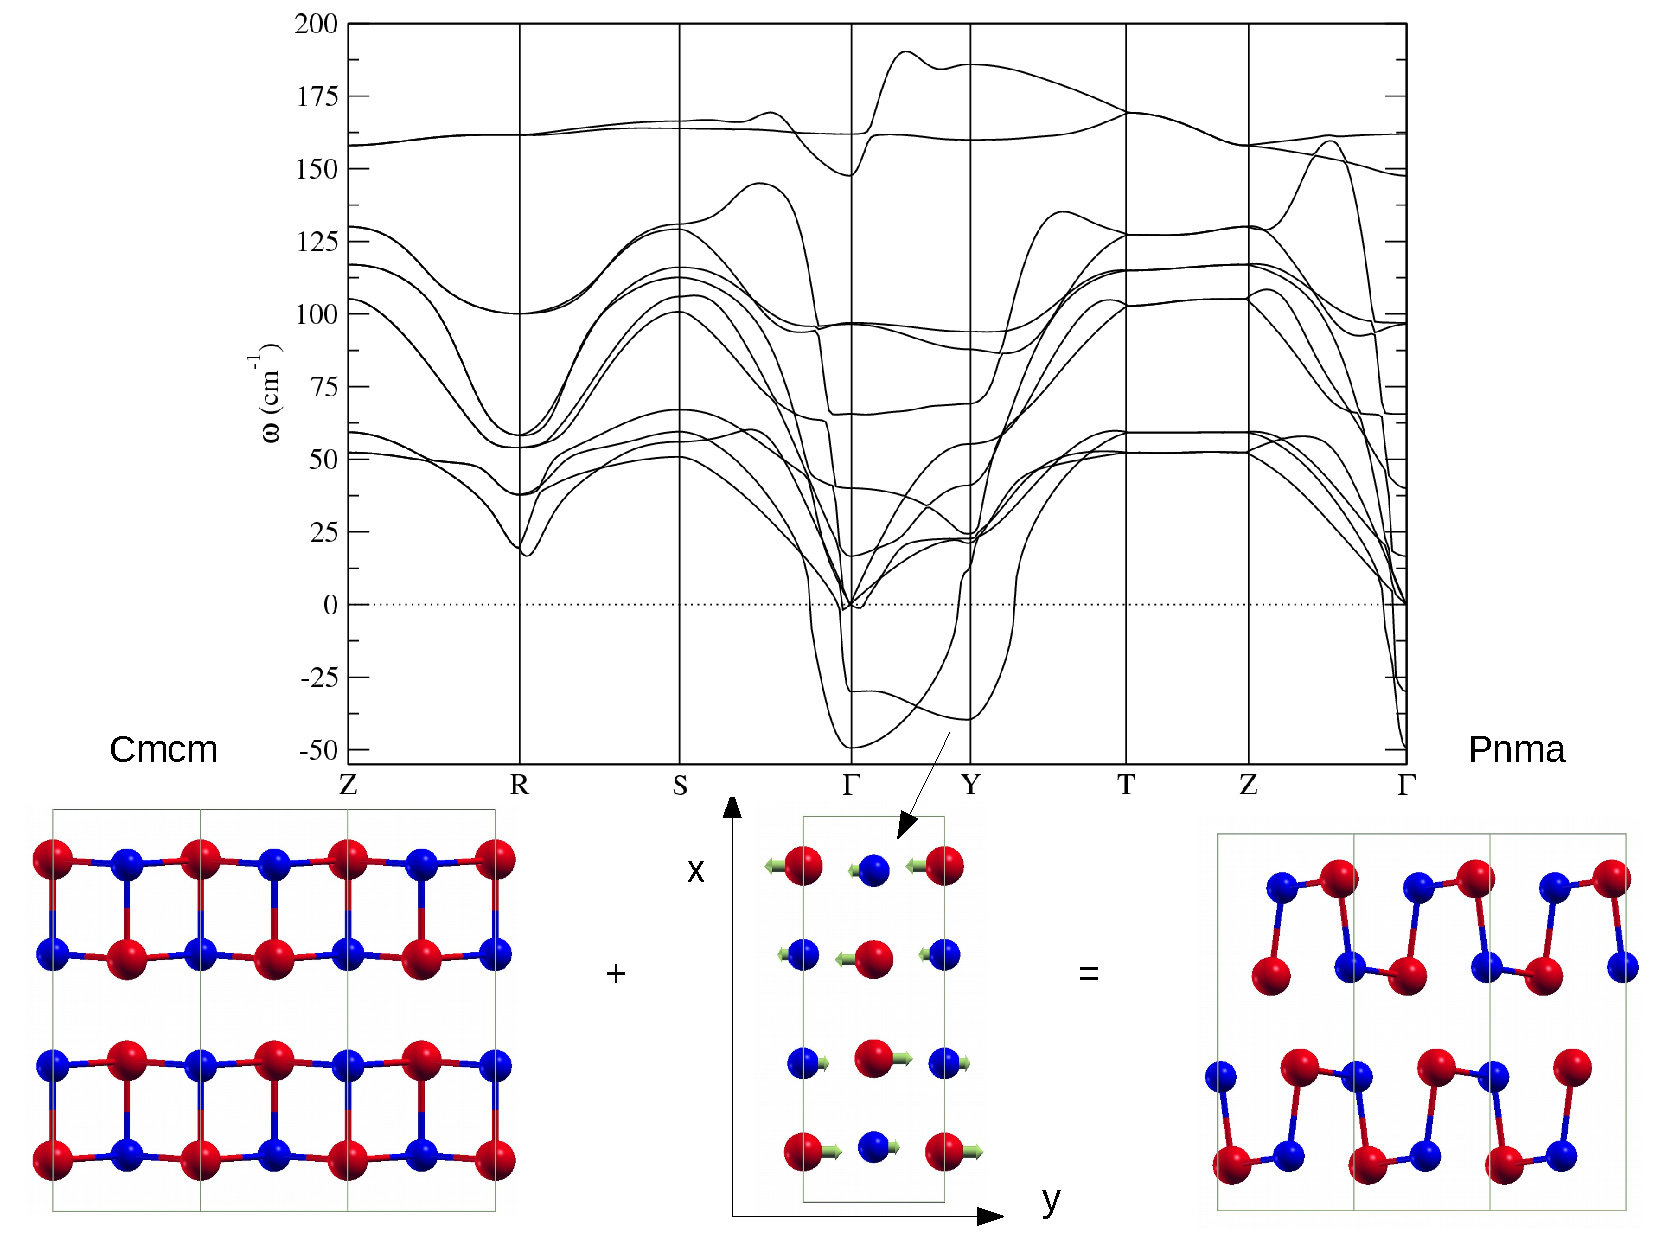
\includegraphics[width=0.7\linewidth]{Pictures/SnSe/figure3.pdf}
\end{center}

\end{frame}

%%%%%%%%%%%%%%%%%%%%%%%%%%%%%%%%%%%%%%%%%%%%%%%%%%%%%%%%%%%%%%%%%%%%%%%%%%%%%%%%%%%%%%%%%%%%%%%%

\begin{frame}

\frametitle{SnSe}
\begin{center}
  \includegraphics[width=0.85\linewidth]{Pictures/SnSe/freq-main.eps}
\end{center}

\end{frame}

%%%%%%%%%%%%%%%%%%%%%%%%%%%%%%%%%%%%%%%%%%%%%%%%%%%%%%%%%%%%%%%%%%%%%%%%%%%%%%%%%%%%%%%%%%%%%%%%

\begin{frame}

 \frametitle{SnSe}
 \vspace{-0.5cm}
 \begin{center}
  \includegraphics[width=0.75\linewidth]{Pictures/SnSe/data-case.eps}
 \end{center}
 \begin{itemize}
  \item We discard the first-order phase transition.
 \end{itemize}

\end{frame}

%%%%%%%%%%%%%%%%%%%%%%%%%%%%%%%%%%%%%%%%%%%%%%%%%%%%%%%%%%%%%%%%%%%%%%%%%%%%%%%%%%%%%%%%%%%%%%%%%%

\end{document}
